\section{Approaches To Property Testing}

  \frame{\sectionpage}

  \begin{frame}{Libraries}
    \begin{table}
      \begin{center}
        \caption{Property Testing Libraries In Various Languages}
        \begin{tabular}{l|S}
             \textbf{Language} & \textbf{Libraries} \\
             \hline
             \multirow{C}{}{} & theft \\
             \hline
             \multirow{C++}{}{} & CppQuickCheck \\
             \hline
             \multirow{Clojure}{}{} & test.check \\
             \hline
             \multirow{Common Lisp}{}{} & cl-quickcheck \\
             \hline
             \multirow{Coq}{}{} & QuickChick \\
             \hline
             \multirow{Erlang}{}{} & QuickCheck \\
             \hline
             \multirow{F\#}{}{} & FsCheck \\ & Hedgehog \\
             \hline
             \multirow{Golang}{}{} & gopter \\ & quick \\
        \end{tabular}
      \end{center}
    \end{table}
  \end{frame}
  
  \begin{frame}{Libraries (Cont'd)}
    \begin{table}[h!]
      \begin{center}
        \caption{Property Testing Libraries In Various Languages}
        \begin{tabular}{l|S}
             \textbf{Language} & \textbf{Libraries} \\
             \hline
             \multirow{}{}{Haskell} & QuickCheck \\ & Hedgehog \\ & Validity \\ & SmallCheck \\
             \hline
             \multirow{}{}{Java} & QuickTheories \\
             \hline
             \multirow{}{}{Javascript} & jsverify \\
             \hline
             \multirow{}{}{PHP} & Eris \\
             \hline
             \multirow{}{}{Python} & Hypothesis \\
             \hline
             \multirow{}{}{Ruby} & Rantly \\
             \hline
             \multirow{}{}{Rust} & QuickCheck \\
             \hline
             \multirow{}{}{Scala} & ScalaCheck \\
             \hline
             \multirow{}{}{Swift} & SwiftCheck \\
             \hline
        \end{tabular}
      \end{center}
    \end{table}
  \end{frame} 

  \begin{frame}[fragile]{QuickCheck}
      \begin{itemize}
          \item Pioneer of randomised property testing
          \item uses `Arbitrary` typeclass for things that can be generated
          \item uses `Testable` typeclass for things that are testable
      \end{itemize}
      
      \begin{minted}[fontsize=\footnotesize]{haskell}
      class Arbitrary a where
        arbitrary :: Gen a
        shrink :: a -> [a]
      \end{minted}
 
      Example:
      \begin{minted}[fontsize=\footnotesize]{haskell}
      λ> quickCheck $ \(str :: String) -> reverse (reverse str) == str
      \end{minted}
  \end{frame}

  \begin{frame}[fragile]{QuickCheck (Cont'd)}
     \begin{minted}[fontsize=\footnotesize]{haskell}
     reflexive :: Arbitrary a => (a -> a -> Bool) -> Property
     reflexive rel = \x -> x `rel` x 
     \end{minted}
     
     But there's a problem:
     \begin{itemize}
         \item This combinator can only test reflexivity of a given binary relation
               if the relation is reflexive for \textit{all} possible values that
               may be generated by the arbitrary generator.
     \end{itemize}
    
     This is already a problem with `Rational` and `Eq`. The `Eq` instance for `Ratio a`
     assumes that values are normalised:
     
     \begin{minted}[fontsize=\footnotesize]{haskell}
     > 2 :% 2 == 1 :% 1
     False
     \end{minted}
     
  \end{frame}

  \begin{frame}{Problems With QuickCheck}
      `Abitrary` is a lawless typeclass, with no precise semantics!
      
      How should we implement the `Arbitrary` instance for `Rational`?:
      
      \begin{itemize}
          \item Should we ever let it generate 0 :\% 0?
          \item Should we ever let it generate 1 :\% 0?
          \item Should we ever let it generate 5 :\% -1? How about -5 :\% 1?
          \item Should we take the size parameter into account?
      \end{itemize}
      
      There are several considerations:
      
      \begin{itemize}
          \item Never generating un-normalised values could fail to test edge-cases
          \item Generating un-normalised values means we cannot test properties that require (==) to work properly
      \end{itemize}
      
      Solution: newtype wrappers?
      
      But there's a limitation there too...
  \end{frame}

  \begin{frame}{Problems with QuickCheck (Cont'd)}
      \begin{itemize}
          \item Expensive generators and shrinking
          \item QuickCheck docs: "There is no generic arbitrary implementation included because we don't know how to make a high-quality one."
          \item There is no default implementation of `arbitrary`
          \item The default implementation of shrink is `const []`. This means that by default, values are never shrunk!
          \item Developers must implement shrinking themselves, which costs developer time. Moreover, test code is already among the most sloppy, hastily written
          code in most any given codebase.
          \item Orphan instances for `Arbitrary`
      \end{itemize}
  \end{frame}
  
  \begin{frame}[fragile]{Hedgehog}
      \begin{itemize}
          \item Very new approach to property testing (Stanley, J. 2017)
      \end{itemize}
      
      \begin{minted}[fontsize=\footnotesize]{haskell}
      import Hedgehog
      import qualified Hedgehog.Gen as Gen
      import qualified Hedgehog.Range as Range
      
      prop_reverse :: Property
      prop_reverse = property $ do
        xs <- forAll $ Gen.list (Range.linear 0 100) Gen.alpha
        reverse (reverse xs) === xs
      \end{minted}
  \end{frame}
  
  \begin{frame}[fragile]{Hedgehog}
      \begin{itemize}
          \item Free shrinking: Paired with every generator internally
          \item Shrinks are represented as a lazy tree which just needs to be traversed for consecutive shrinks
          \item Much prettier/clearer output, with source
      \end{itemize}
  \end{frame}
  
  \begin{frame}[fragile]{Hedgehog}
      \begin{minted}[fontsize=\footnotesize]{haskell}
      import Hedgehog
      import qualified Hedgehog.Gen as Gen
      import qualified Hedgehog.Range as Range
      import qualified Data.List as List
     
      genIntList :: Gen [Int]
      getIntList =
        let listLength = Range.linear 0 10_000
        in Gen.list listLength Gen.enumBounded
      
      prop_reverse :: Property
      prop_reverse = property $ do
        xs <- forAll genIntList
        reverse (reverse xs) == xs
      
      -- λ> check prop_reverse
      -- ✓ prop_reverse passed 100 tests.
      \end{minted}
  \end{frame}
 
  \begin{frame}[fragile]{Hedgehog}
     Let's do what I do best and write some bad code...
     \begin{minted}[fontsize=\footnotesize]{haskell}
     -- Drops an element somewhere around the middle of the list.
     fauxReverse :: [a] -> [a]
     fauxReverse xs =
       let sx = List.reverse xs
           mp = length xs `div` 2
           (as, bs) = List.splitAt mp sx
       in as <> List.drop 1 bs

     prop_fauxReverse :: Property
     prop_fauxReverse =
       property $ do
         xs <- forAll genIntList
         fauxReverse xs === List.reverse xs
     \end{minted}
  \end{frame}
    
  \begin{frame}[fragile]{Hedgehog}
     And now we test my bad code...
     \begin{center}
     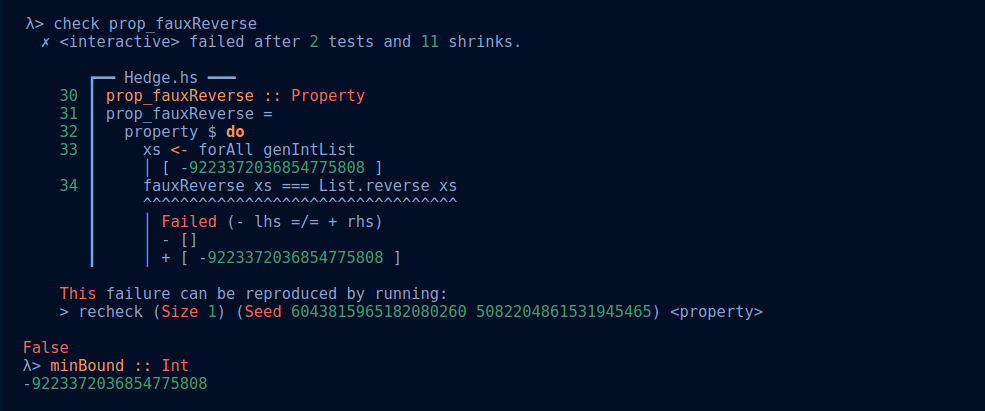
\includegraphics[width= 1.0\textwidth]{images/hedgehog_faux_reverse_output.png}
     \end{center}
  \end{frame}
  
  \begin{frame}[fragile]{Hedgehog}
      \begin{minted}[fontsize=\footnotesize]{haskell}
      -- A reverse function should preserve every element in the list!
      prop_fauxReverseLength :: Property
      prop_fauxReverseLength = property $ do
        xs <- forAll genIntList
        length (fauxReverse xs) === length xs 
      \end{minted}
     
      \begin{center}
      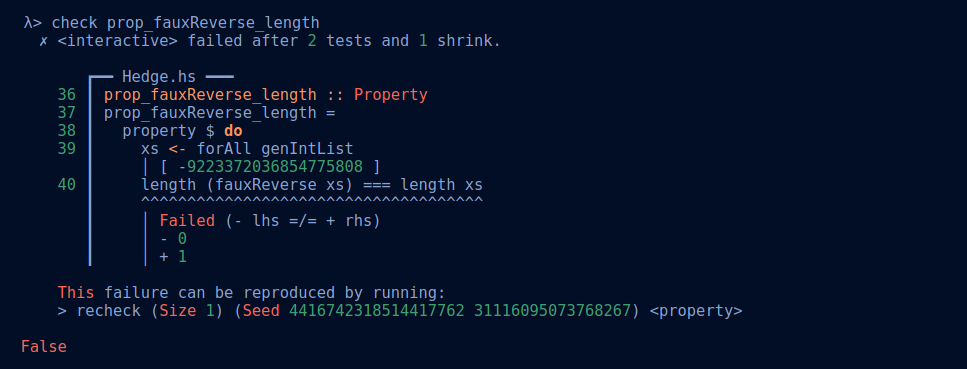
\includegraphics[width= 1.0\textwidth]{images/hedgehog_faux_reverse_length_output.png}
      \end{center} 
  \end{frame}